\section{Background}

%The ultimate assessment standard for knowledge is its ability to inform action.
%As such, neuroscience incrementally aims to support the development of meaningful and predictable control of the brain.
%Within this endeavour, it is the most easily accessible components of the brain, given current technology, which can provide the greatest opportunities for advancement.

The dopaminergic system consists of a strongly localized, and widely projecting set of neurons (\cref{fig:ml}).
On account of the small number of dopaminergic neurons ($\approx300,000$ in humans \cite{rice2016}, $\approx10,000$ in rats \cite{german1993}, and $\approx4,000$ in mice \cite{triarhou1988}), tractography commonly fails to resolve the degree centrality of the dopaminergic system, and thus it is not commonly depicted as a significant network node.
However, it is precisely the small number of widely branching and closely similar neurons, which makes the dopaminergic system a credible candidate for truly node-like function in coordinating brain activity.
As is expected given such salient features, the system is widely implicated in neuropsychiatric phenomena (including
addiction \cite{DiChiara1988,DiChiara1999},
attentional control \cite{Nieoullon2002},
motivation \cite{Salamone1994},
creativity \cite{Chermahini2010},
personality \cite{Depue1999},
neurodegeneration \cite{Masliah2000},
and schizophrenia \cite{Howes2009}),
and is a common target for pharmacological interventions.
Manipulation of the dopaminergic system extends widely beyond the medical field, and includes performance-enhancing \cite{Mehta2000,Turner2003}, as well as recreational usage \cite{DiChiara1988}.
As such, better and more predictively powerful models of the dopaminergic system can enhance numerous aspects of human activity, in the clinic and beyond.

\begin{sansmath}
\begin{figure*}[h!]
	\centering
	\hspace*{\fill}
	\begin{subfigure}{.527\textwidth}
		\centering
		\vspace{-1em}
		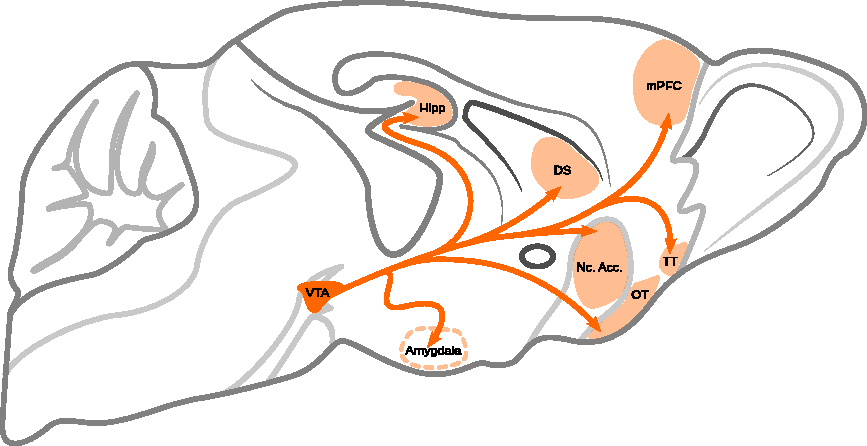
\includegraphics[width=\textwidth]{img/model_literature}
		\caption{
			Schematic map of VTA dopaminergic projections \cite{Aransay2015,Fields2007,Ikemoto2007,Hnasko2012,Pan2010}.
			Dotted structures are off-slice, and projection arrows do not reflect actual fiber bundle paths.
			Abbreviations: Hipp (Hippocampus), DS (Dorsal Striatum), NAcc (Nucleus Accumbens), OT (Olfactory Tuberculum), mPFC (medial Prefrontal Cortex), TT (Tenia Tecta).
			}
		\label{fig:ml}
	\end{subfigure}\hfill
	\begin{subfigure}{.44\textwidth}
		\centering
		\vspace{-2em}
		\includedot[width=1.1\textwidth]{data/network_model}
		\vspace{-2em}
		\caption{
			Simplified network model of 1-step signal relay following optogenetic stimulation of the VTA.
			The $\mathrm{u_1}$ weighting corresponds to VTA somatic excitability and $\mathrm{u_{2a},u_{2b},u_{2c}}$ and $\mathrm{u_{2d}}$ correspond to transmission at the dopaminergic synapses in the respective projection areas.
			}
		\label{fig:nm}
	\end{subfigure}
	\hspace*{\fill}
	\begin{subfigure}{.985\textwidth}
		\centering
		\vspace{.5em}
		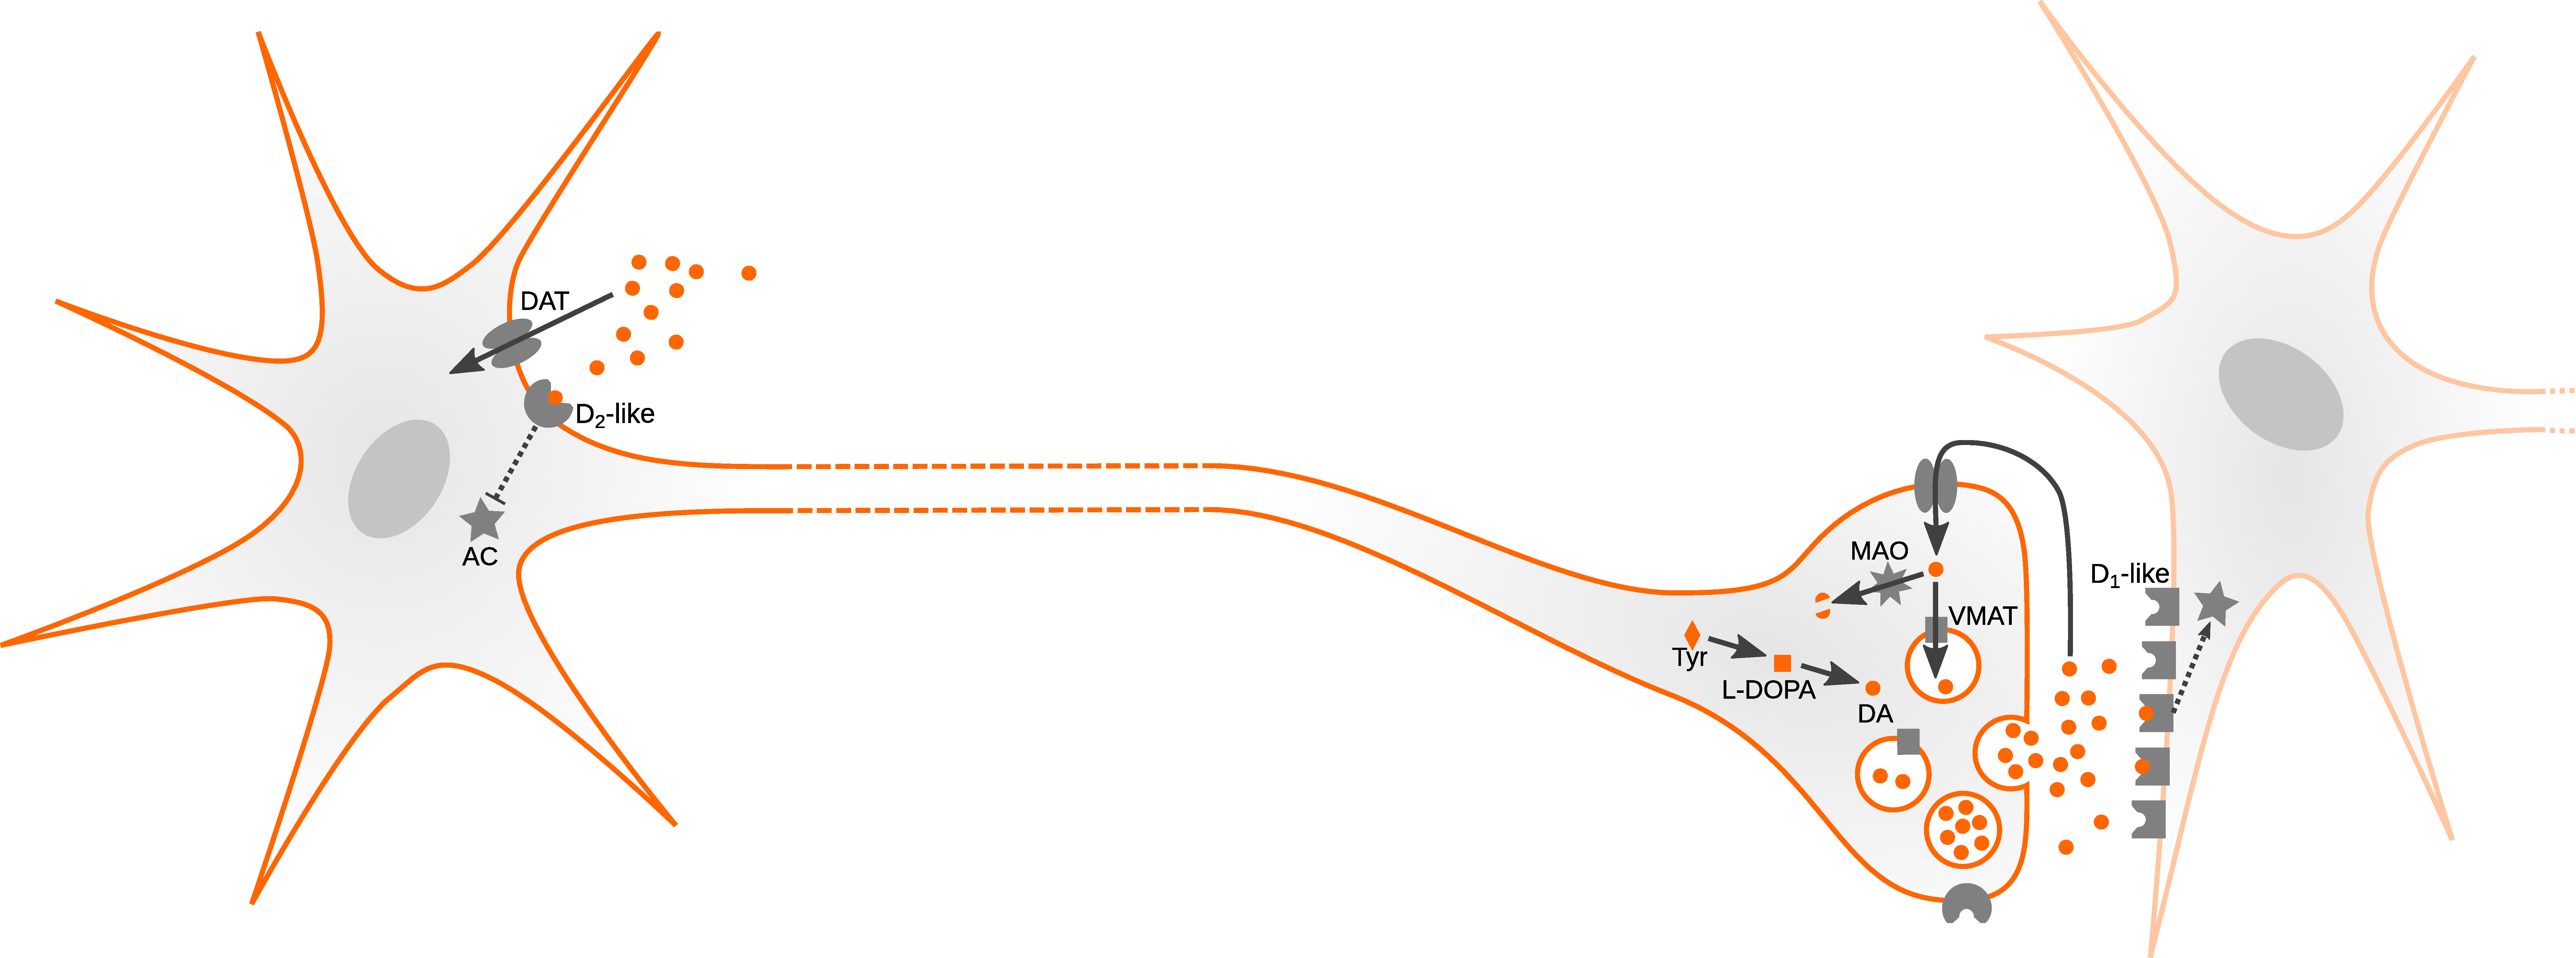
\includegraphics[width=\textwidth]{img/da}
		\caption{
			Schematic overview of VTA dopaminergic neurons, with the soma located in the VTA and synapses in one or multiple other projection area voxels.
			Excitability at the soma are contingent on $\mathrm{D_2}$ autoinhibition, while transmission at the synapse is contingent on dopamine metabolism, turnover, and postsynaptic $\mathrm{D_1}$ expression.
			Abbreviations: AC (adenylyl cyclase), DA (dopamine), DAT (dopamine transporter), MAO (monoamine oxydase), VMAT (vesicular monoamine transporter), Tyr (tyrosine) \cite{Torres2003}.
			}
		\label{fig:cm}
	\end{subfigure}
	\begin{subfigure}{.985\textwidth}
		\centering
		\vspace{.5em}
		\includegraphics[width=0.95\textwidth]{img/optogenetics}
		\caption{
			Schematic of optogenetic cell selection and activation.
			Orange denotes dopaminergic cells, gray enlarged elements on the cell periphery indicate channelrhodopsin expression, and cyan segments on the cell periphery denote depolarization events.
			}
		\label{fig:og}
	\end{subfigure}
	\caption{
		\textbf{The cell biological compartmentalization of dopaminergic neurotransmission (and susceptibility to psychopharmacology) can partly be mapped onto neuroanatomical features by a simple network model, using optogenetics.}
		Depicted are schematic overviews of the VTA dopaminergic system at various spatial resolutions.
		}
	\label{fig:m}
\end{figure*}
\end{sansmath}

Experimentation in human subjects is methodologically constrained, and thus neuroscience relies on other methods, such as model animal research, for cell biological insights, which are instrumental to the refinement of interventions.
Due to high evolutionary conservation \cite{Yamamoto2011}, the dopaminergic system is an excellent candidate for translational study.
Of the common model animals, the mouse offers significant advantages including short generation spans, broad availability of transgenic lines, highly accessible histology, and the smallest size among mammalian model organisms.
Far from trivial, this latter quality offers a significant advantage for numerous imaging techniques, including optics, optoacoustics, and magnetic resonance imaging (MRI).
Furthermore, the small size greatly increases experiment scalability and multi-center reproducibility, beyond even what can be acchieved using the rat model.
Of particular relevance to pharmacological research, the mouse possesses a high metabolic rate, allowing for rapid drug clearance and thus high contrast in repeated drug administration sessions.

As it coordinates phenomena such as perception, decision, and action, the function of the brain is highly holistic, suggesting the use of whole-brain measurement techniques for its characterization.
This is particularly true for monoaminergic neurotransmitter systems, where focal interventions can have wide-ranging effects.
Owing to its deep penetration, high rostrocaudal coverage, and large-scale usage in human studies, fMRI is one of the foremost methods for studying dopaminergic modulation of brain function.

Imaging a neurotransmitter system comprised of a small number of cells, based only on spontaneous activity, is highly unreliable due to a very low signal to noise ratio (SNR).
This limitation can, however, be overcome by introducing exogenous stimuli.
While the colocalization of widely projecting dopaminergic cell bodies into nuclei makes targeting comparatively easy, dopaminergic nuclei also contain notable populations of non-dopaminergic cells.
Activating such cells may confound an intended dopaminergic read-out, as they exhibit different kinetics, especially with regard to psychopharmacology \cite{Taylor2014}.
In order to specifically target dopaminergic cells, they need to be sensitized to an otherwise inert stimulus in a transcription-dependent manner.
This can be achieved via optogenetics, a method based on light-stimulation of cells expressing light-sensitive proteins such as channelrhodopsin \cite{Boyden2005}.
Cell-type selectivity can be achieved by Cre-conditional channelrhodopsin vector delivery \cite{Orban1992} to transgenic animals expressing Cre-recombinase under a dopaminergic promoter.
Following protein expression, stimulation can be delivered via an implanted optic fiber.
The combination of this stimulation method with fMRI is commonly referred to as opto-fMRI \cite{Desai2011,Grandjean2019}.

The dopaminergic system is centralized in the midbrain and consists of two lateralized nucleus pairs, the Ventral Tegmental Area (VTA) and Substantia Nigra pars compacta (SNc).
Of these, the VTA displays a wider distribution of efferents (\cref{fig:ml}), whereas the SNc projects primarily to the dorsal striatum \cite{Pan2010}.

The most popular means of producing spatially resolved sensitivity summaries from fMRI, and opto-fMRI in particular, is general linear modelling (GLM) of stimulus evoked activity \cite{Friston1995}.
For this purpose, a precisely specified stimulus train is presented to the brain, and convolved with an impulse response function (IRF, also called hemodynamic response function) for analysis.
Subsequently, a mass univariate regression analysis is performed across all voxels, allowing them to be assigned parameter values, which denote the strength of activation adjusted for the sample noise.
While powerful, this approach implies that all voxels in the brain are exposed in an indistinguishable fashion to the stimulation, a questionable assumption in view of the actual network architecture.
Particularly in cases where stimulation is introduced via well-known pathways, a simple network model for signal transmission could be explored via seed-based functional connectivity (\cref{fig:nm}).
Moreover, for neurotransmitter systems with colocalized cell bodies and long efferent projections, the macroscopic resolution of fMRI allows mapping somatodendritic processes (e.g. excitability upon depolarization at the soma) to “cell-body“ voxels, and signal transmission at the synapse to “projection“ voxels (\cref{fig:cm}).

This study pertaining to whole-brain modelling of human VTA dopaminergic function in mice aims to produce three novel research outputs.
Firstly, proof-of-principle documenting the feasibility of dopaminergic VTA opto-fMRI in the mouse should be demonstrated, and a reference dataset published.
Secondly, controlled methodological variation effects should be described and evaluated, to lay a reliable and well-informed foundation for the technique, allowing its reuse as a general-purpose dopaminergic system assay.
Lastly, a voxelwise summary of dopaminergic function in the healthy adult mouse should be published in a standard volumetric space, to facilitate co-registered data integration, operative targeting, and comparative evaluation of treatment or pathology induced effects.
